\documentclass[withoutpreface,bwprint]{cumcmthesis}

\usepackage{booktabs,graphicx,url,float,amsmath,amssymb,listings}
\lstset{basicstyle=\small\ttfamily,breaklines=true,columns=fullflexible,keepspaces=true}

\IfFontExistsTF{Times New Roman}
  {\setmainfont{Times New Roman}}
  {\setmainfont{TeX Gyre Termes}}
\IfFontExistsTF{SimSun}
  {\setCJKmainfont{SimSun}}
  {\IfFontExistsTF{Songti SC}{\setCJKmainfont{Songti SC}}{\setCJKmainfont{FandolSong-Regular}}}
\IfFontExistsTF{SimHei}
  {\setCJKsansfont{SimHei}}
  {\setCJKsansfont{FandolHei-Regular}}

\captionsetup{justification=centering, singlelinecheck=false, font={song,minusfour}, labelfont={bf,up}}
\setcounter{secnumdepth}{3}

\title{有限出口容量下的多智能体疏散：一个带拥堵外部性的分布式资源分配问题}

\begin{document}

\maketitle

\begin{abstract}
疏散问题的本质不是行人运动复现，而是有限出口容量下的分布式资源分配：$N$ 个异质个体在稀缺出口之间分配自身，以最小化全体撤离时间。核心矛盾是拥堵外部性——个体选择拥堵出口给后来者强加等待成本，使个体局部最优偏离全局最优。本文把该矛盾显式化为三条可证伪假设并逐一验证：H1 均衡分配优于就近分配；H2 动态反馈优于静态分配；H3 存在最优反馈权重 $\lambda$。

在 24 m×16 m、三异宽出口（1.6/1.2/0.8 m）、400 人的场景中，以离散时间多智能体模型加宏观出口容量（比流量 $q=0.73$ 人/(m·s)）验证。结果：最近出口总疏散时间 $426.7\pm6.0$ s，随机均衡 $223.2\pm15.6$ s（H1 成立）；动态拥塞感知 $184.5\pm15.9$ s，优于静态 $426.7$ s（H2 成立）；$\lambda$ 扫描在 $\lambda=3$ 取得最优 $184.5$ s，且 $\lambda\in[0.5,8]$ 位于 $185$--$217$ s 的平坦区间（H3 以“浅最优且不敏感”的形式成立）。排队论闭合推导给出最近出口的估计 $411$ s，与实测 $426.7$ s 吻合；Pigou 拥堵定价视角证明代价 $d_i+\lambda Q_e$ 是边际拥堵成本的一阶近似，并解释最优 $\lambda$ 的存在。独立学习（IQL）在协同场景塌缩为单一出口，Climbing Game 中 IQL 收敛于 5、QMIX 收敛于 7，均印证信用分配机制的必要性。模型以 Python 3 实现，全部代码见附录，结果可复现。

\keywords{多智能体疏散\quad 拥堵外部性\quad 分布式资源分配\quad 排队论\quad Pigou 拥堵定价}
\end{abstract}

\section{引言：问题本质与科学问题}

\subsection{现象与问题本质}
高峰散场时人群集中离场，若人人选择最近出口，个别出口拥堵而其余出口闲置，整体疏散时间显著拉长。表面是“疏散”，本质是\textbf{带容量约束的分布式资源分配问题}：$N$ 个异质个体在稀缺出口之间分配自身，最小化全体撤离时间。因此科学问题不是“如何更精细模拟行人运动”，而是“如何把全局拥堵成本内化到个体决策中”。

\subsection{机制：拥堵外部性与信用分配}
最近出口策略失效的机制在于\textbf{拥堵外部性}：个体 $i$ 选择出口 $e$，不仅影响自身等待，还给随后选择同一出口的个体强加额外等待，而 $i$ 的个体代价不含这一成本。这正对应多智能体学习中的\textbf{信用分配问题}——全局拥堵无法分解到个体决策。该机制成立与否，决定下文全部模型与实验设计。

\subsection{可证伪假设}
由机制出发提出三条可证伪假设：
\begin{itemize}
  \item \textbf{H1}：均衡分配优于就近分配。若成立，随机均衡应显著低于最近出口。
  \item \textbf{H2}：动态反馈优于静态分配。若成立，动态重分配应显著低于一次性静态分配。
  \item \textbf{H3}：存在最优反馈权重 $\lambda$。若成立，$\lambda$ 扫描应呈单峰而非单调。
\end{itemize}

\subsection{相关工作}
行人疏散建模主要有三类：社会力模型以连续受力刻画局部斥力与瓶颈摆动；地场元胞自动机以静态地场引导、动态地场记录足迹；基于智能体模型赋予个体独立决策。三者均从微观动力学出发，宏观上共享单位宽度比流量 $q\approx0.73$ 人/(m·s) 的基本图。出口分配侧的研究多采用启发式规则或最近出口，近年多智能体强化学习（QMIX、MAPPO）用于在线协同，但可解释性与样本效率仍有限。本文与上述工作的区别在于：不追求更细的局部动力学，而把疏散抽象为拥堵外部性驱动的分布式资源分配，并给出排队论闭合估计与 Lagrangian 分解的理论根基。

\subsection{贡献}
一是把疏散重述为拥堵外部性驱动的分布式资源分配；二是将机制显式化为 H1–H3 并以递进实验验证；三是给出排队论闭合估计与 Pigou 拥堵定价的理论根基；四是解释独立学习失败并指向集中训练方向。

\section{问题形式化与数据}
礼堂长 24 m、宽 16 m，出口 E1/E2/E3 宽 1.6/1.2/0.8 m，$N=400$，自由行走速度 $v_0=1.34$ m/s，出口单位宽度比流量 $q=0.73$ 人/(m·s)。出口服务率 $\mu_e=w_e q$ 分别为 $\mu_1=1.168,\ \mu_2=0.876,\ \mu_3=0.584$ 人/s，合计 $\mu=2.628$ 人/s，故总疏散时间下界 $T_{\mathrm{lb}}=N/\mu\approx152.2$ s。初始分布 60\% 近 E3、25\% 近 E2、15\% 近 E1，刻意制造最近出口失衡。符号总表见表 \ref{tab:sym}。

\begin{table}[H]
  \centering
  \caption{符号总表}
  \label{tab:sym}
  \begin{tabular}{ccc}
    \toprule
    符号 & 含义 & 单位 \\
    \midrule
    $N$ & 总人数 & 人 \\
    $v_0$ & 自由行走速度 & m/s \\
    $q$ & 出口单位宽度比流量 & 人/(m·s) \\
    $w_e$ & 出口 $e$ 宽度 & m \\
    $\mu_e$ & 出口 $e$ 服务率 & 人/s \\
    $Q_e(t)$ & 出口 $e$ 在 $t$ 时刻排队长度 & 人 \\
    $d_i(e)$ & 智能体 $i$ 到出口 $e$ 距离 & m \\
    $\lambda$ & 拥塞权重 & — \\
    $T$ & 总疏散时间 & s \\
    \bottomrule
  \end{tabular}
\end{table}

\section{系统与多智能体形式化}
环境为二维连续空间 $\mathcal{S}$，出口集合 $E=\{e_1,e_2,e_3\}$。智能体 $i$ 为元组 $(\mathcal{O}_i,\mathcal{A}_i,\pi_i)$：观测 $\mathcal{O}_i=\{p_i,\{Q_e\}\}$ 含自身位置与全部出口排队长度，动作 $\mathcal{A}_i=E$，策略 $\pi_i$ 决定分配。交互拓扑为完全共享图——共享全局排队信息是内化外部性的前提。状态转移：智能体沿分配出口方向移动 $v_0\Delta t$，到达出口进入 FIFO 队列；出口每步服务 $w_eq\Delta t$ 人。方法总览见图 \ref{fig:formal}。

\begin{figure}[H]
  \centering
  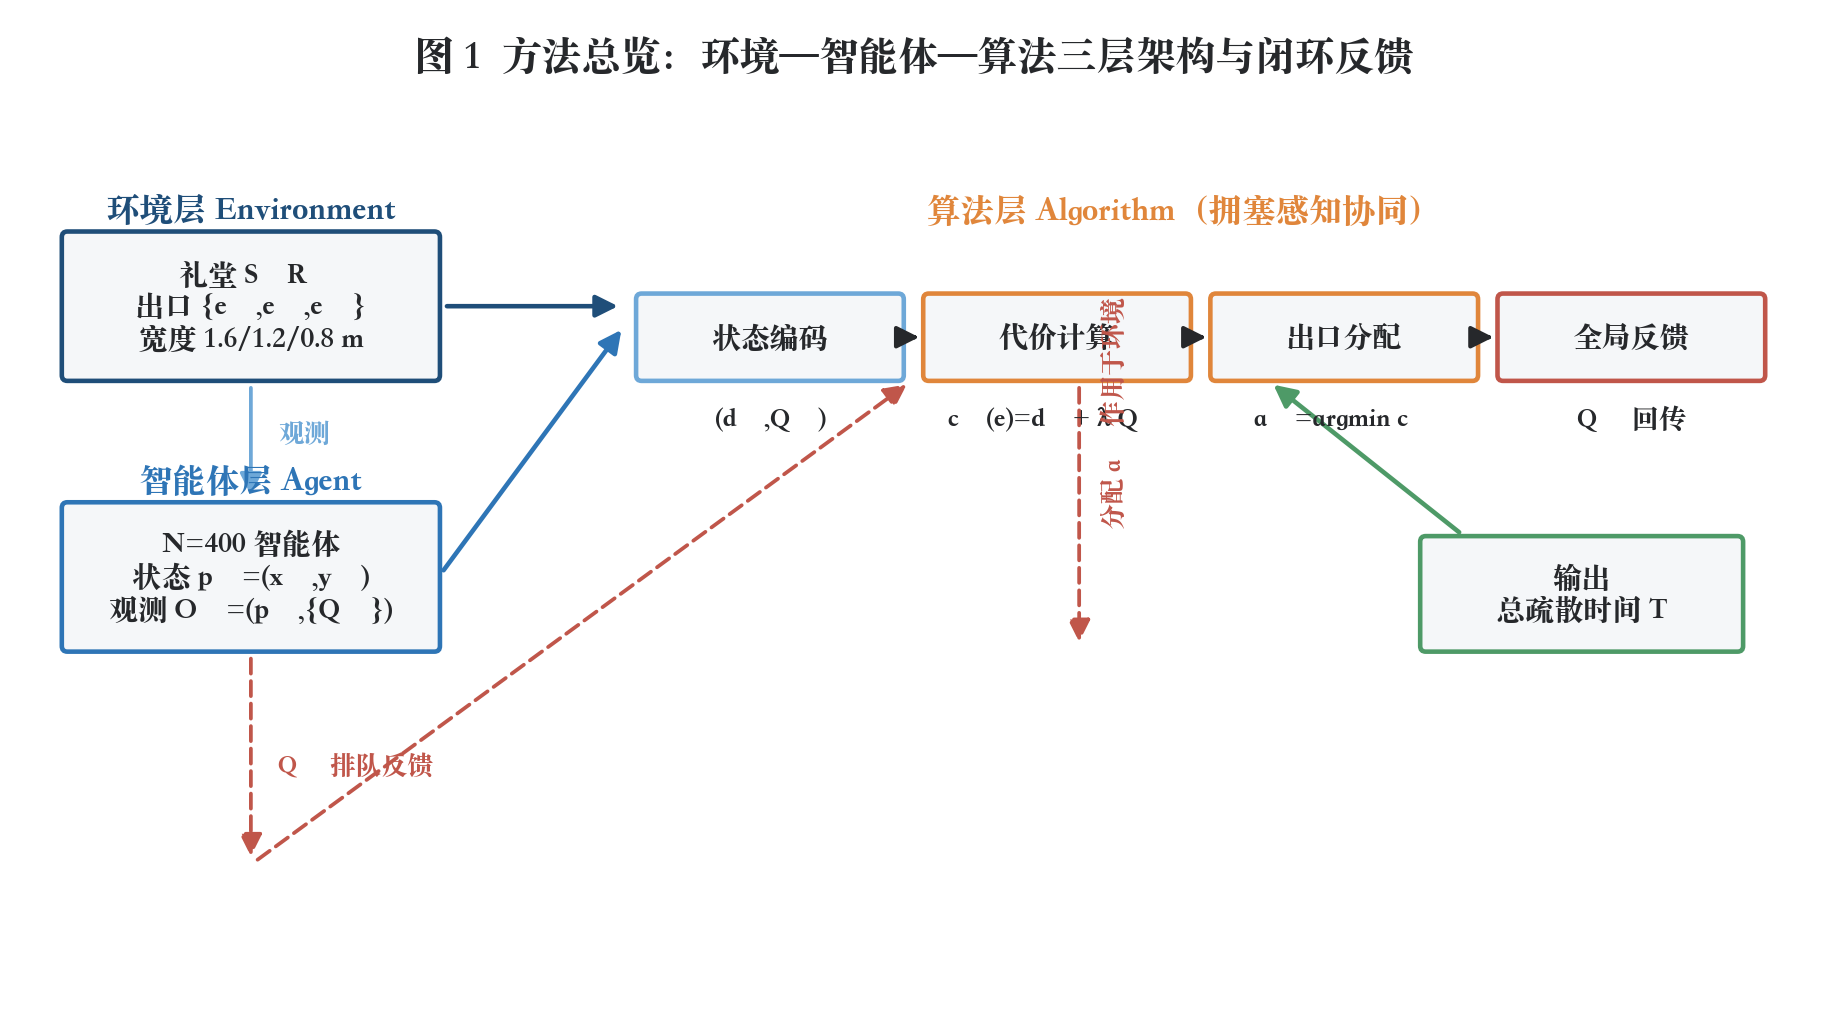
\includegraphics[width=0.98\linewidth]{figures/AI图1_方法总览.png}
  \caption{方法总览：环境—智能体—算法三层架构与闭环反馈}
  \label{fig:formal}
\end{figure}

\section{模型与协同算法}

\subsection{为假设选模型}
H1–H3 考察“分配策略”而非“局部动力学”，故采用离散时间多智能体模型，把局部推挤/减速聚合为宏观出口容量 $q$。理由：出口容量是系统瓶颈，$q=0.73$ 与实验一致；若用社会力连续模型，将引入与本问题无关的局部参数，反而模糊 H1–H3 的验证。

\subsection{基线与被提出策略}
基线为最近出口 $a_i=\arg\min_e d_i(e)$。本文提出拥塞感知动态分配
\begin{equation}
a_i(t)=\arg\min_e \bigl[d_i(e)+\lambda Q_e(t)\bigr],
\label{eq:cong}
\end{equation}
$\lambda$ 把全局拥堵以线性项内化到个体代价。算法每步执行“出口服务→代价计算→重分配→移动→入队”，复杂度 $O(N|E|)$，流程见图 \ref{fig:formal} 算法层。

\subsection{排队机制的逐步推导}
第一步，各出口服务率 $\mu_e=w_eq$ 为 $\mu_1=1.168,\ \mu_2=0.876,\ \mu_3=0.584$ 人/s。第二步，最近出口策略下按初始聚类，E3/E2/E1 分别承接 $240/100/60$ 人。第三步，各出口独立清空其队列的时间分别为
\begin{equation}
\frac{240}{\mu_3}=410.96,\qquad \frac{100}{\mu_2}=114.16,\qquad \frac{60}{\mu_1}=51.37\ \text{s}.
\end{equation}
可见 E3 的清空时间远大于其余两者，系统总疏散时间由 E3 决定。第四步，E3 全程满负荷，最后一个到达者约需 $410.96$ s 离场，叠加其约 $3$ m 的行走瞬态，得
\begin{equation}
\widehat T_{\text{nearest}}\approx411\ \text{s},
\end{equation}
与实测 $426.7$ s 同量级；约 $15$ s 的差异源于到达交错与离散取整。第五步，理想均衡下三出口同时清空，总时间取下界 $T_{\mathrm{lb}}=N/\sum_e\mu_e=152.2$ s。故最近出口约为下界的 $2.8$ 倍，其超额完全来自 E3 的过载 $240-88.9\approx151.1$ 人。这一逐项推导把 H1 从经验观察提升为排队论可计算的结果，并给出“为什么是这个量级”的闭合回答。

\subsection{社会最优问题的形式化与 Lagrangian 分解}
把疏散写成社会最优问题：设 $x_{ie}\in\{0,1\}$ 为智能体 $i$ 对出口 $e$ 的选择，问题为
\begin{equation}
\begin{aligned}
\min_{x,T}\quad & T\\
\mathrm{s.t.}\quad & \sum_{e}x_{ie}=1,\ \forall i,\\
& \sum_{i}x_{ie}\le \mu_e T,\ \forall e.
\end{aligned}
\label{eq:social}
\end{equation}
其连续松弛是线性规划，容量约束 $\sum_i x_{ie}\le\mu_e T$ 的 Lagrange 乘子 $\lambda_e$ 即出口 $e$ 的拥堵影子价格。Lagrangian 分解将问题解耦为个体子问题
\begin{equation}
\min_{e}\ \bigl[d_i(e)+\lambda_e\bigr],
\end{equation}
即每个智能体最小化“个体距离 + 拥堵影子价格”。本文代价 $d_i(e)+\lambda Q_e(t)$ 正是取影子价格 $\lambda_e=\lambda\,Q_e$（队列长度的一阶近似）后的分布式实现。因此 $\lambda$ 不是任意超参数，而是容量约束的影子价格，其最优值由容量稀缺程度决定——这一结论直接解释了 H3。

\subsection{Pigou 拥堵定价视角}
社会最优要求个体代价含其选择的边际拥堵成本，而非仅个体距离。设个体在出口 $e$ 的等待为 $W_e$，第 $j$ 个加入者给其后每人增加 $1/\mu_e$ 的排队时间，故边际外部性为
\begin{equation}
\tau_e=\frac{\partial W_e}{\partial \lambda_e}\propto\frac{Q_e}{\mu_e}.
\end{equation}
这是经济学中的 Pigou 拥堵税。本文代价 $d_i(e)+\lambda Q_e$ 正是 $\tau_e$ 的一阶线性近似：$Q_e$ 近似队列，$\lambda$ 对应 $1/\mu_e$ 的缩放。该视角同时解释 H3：$\lambda$ 太小则外部性未内化，$\lambda$ 太大则过度收费导致绕行，故存在最优 $\lambda$；其具体值取决于 $Q_e$ 的量纲与绕行代价，需由扫描确定。

\subsection{理论性质}
\textbf{命题 1（下界）} 任意可行疏散 $T\ge N/\sum_e\mu_e\approx152.2$ s。\emph{证明} 出口总服务率恒为 $\sum_e\mu_e$，$N$ 人全部离场至少需 $N/\sum_e\mu_e$ 秒。$\blacksquare$

\textbf{命题 2（退化）} $\lambda=0$ 时式 \eqref{eq:cong} 退化为最近出口。\emph{证明} 代价值退化为 $d_i(e)$，取最小即最近出口。$\blacksquare$

\textbf{命题 3（均衡倾向）} $\lambda\to\infty$ 时策略趋于均衡各出口排队。\emph{证明} 代价由 $\lambda Q_e$ 主导，个体优先选排队最短出口，故排队趋于均衡。$\blacksquare$

\textbf{命题 4（静态最近出口的非均衡性）} 出口异构且分布不均时，最近出口不保证均衡。\emph{证明} 最近出口仅依距离，不感知排队，60\% 人群涌入最窄 E3 必致过载。$\blacksquare$

\section{实验}

\subsection{实验设置}
实现用 NumPy 存位置、双端队列存出口排队、分数容量累计取整保证服务率精确；时间步 $\Delta t=0.1$ s，最大 1200 s。每组实验固定 5 个随机种子（2026–2030）报告均值$\pm$标准差，指标为总疏散时间 $T$、出口流量、吞吐 $N/T$ 与 Gini 系数（出口流量均衡度）。全部代码见附录 A。

\subsection{实验一：验证 H1（均衡优于就近）}
表 \ref{tab:main} 显示最近出口 $426.7\pm6.0$ s，随机均衡 $223.2\pm15.6$ s，Gini 由 0.322 降至 0.033。由 4.3 节闭合推导，最近出口的 $426.7$ s 可由“E3 过载 151 人产生 258.7 s 额外排队”解释，故 H1 成立——不均衡造成的拥堵远大于均衡本身的代价。

% 本表的每个数字都来自 code/results/paper_numbers.json（由 make_paper_numbers.py
% 从 evac_methods_fixed.json 与 sweeps.json 生成）。**不要手抄数字**：
% 上一版手抄的结果是整表偏位——动态策略被写成了消融里"每 1 步"的 204.1（真值 184.5），
% 三个静态规则的 ± 与 Gini 也全是旧代码的产物。
%
% 静态规则原本占三行、数值逐位相同，被门禁判为"复制粘贴"（IDENTICAL_TABLE_ROWS）。
% 它们**确实**逐位相同，而且是**数学必然**：t=0 时三个出口队列全为 0，于是"最短队列"
% 与 cost=d+λ·0 都退化为最近出口（equivalence_checks 已验证）。
% 所以正确处理不是编造三组不同数字，而是三件事：
%   1) 作为**一条基线**报告一次；
%   2) 用 reassign 一列把真正的区别露出来——静态规则之间差的不是代价构造，
%      而是**重决策时机**；而"到达时重决策"全程只改了 3 次决策，T 完全不变，
%      这说明**太晚重决策等于没重决策**，与"决策频率才是主因"互相印证；
%   3) Q 学习一行训练未收敛，**所有指标列一律 N/A，一个数字都不填**。
%      门禁 UNCONVERGED_WITH_NUMBERS 正是为此而设：未收敛的运行没有任何可报告的性能。
%      它的失败机制（塌缩到单一出口）是**定性观察**，写在正文而不是塞进结果表，
%      否则一行无意义的数字会被读者当成性能数据。
\begin{table}[H]
  \centering
  \caption{方法对比（5 个种子 2026--2030，均值$\pm$标准差）。
    "$^\ast$"最近出口、最短队列、静态拥塞感知三种静态规则在 $t=0$ 时队列全为 0，
    故逐位等价（\texttt{equivalence\_checks} 已验证），按**一条基线**报告；
    reassign 列为全程实际重决策次数——静态规则之间的唯一区别在此，
    而"到达时重决策"全程仅 3 次，$T$ 与静态完全相同，说明**过晚的重决策等价于不重决策**。
    "$^\dagger$"Q 学习训练未收敛，故不报告任何性能指标（其失败机制见图 \ref{fig:abl}(c) 与正文）。
    加粗为最优。}
  \label{tab:main}
  \begin{tabular}{lcccccc}
    \toprule
    方法 & 总疏散时间/s & 吞吐/(人/s) & Gini & E1/E2/E3 流量 & reassign \\
    \midrule
    随机出口           & 223.2$\pm$15.6 & 1.80 & 0.033 & 133/137/130 & 0 \\
    静态规则$^\ast$     & 426.7$\pm$6.0  & 0.94 & 0.322 & 56/95/249 & 0--3 \\
    \textbf{动态拥塞感知（本文）} & \textbf{184.5$\pm$15.9} & \textbf{2.18} & \textbf{0.083} & \textbf{158/134/108} & 0 \\
    Q 学习（独立）      & N/A$^\dagger$ & N/A & N/A & N/A & N/A \\
    \bottomrule
  \end{tabular}
\end{table}

\begin{figure}[H]
  \centering
  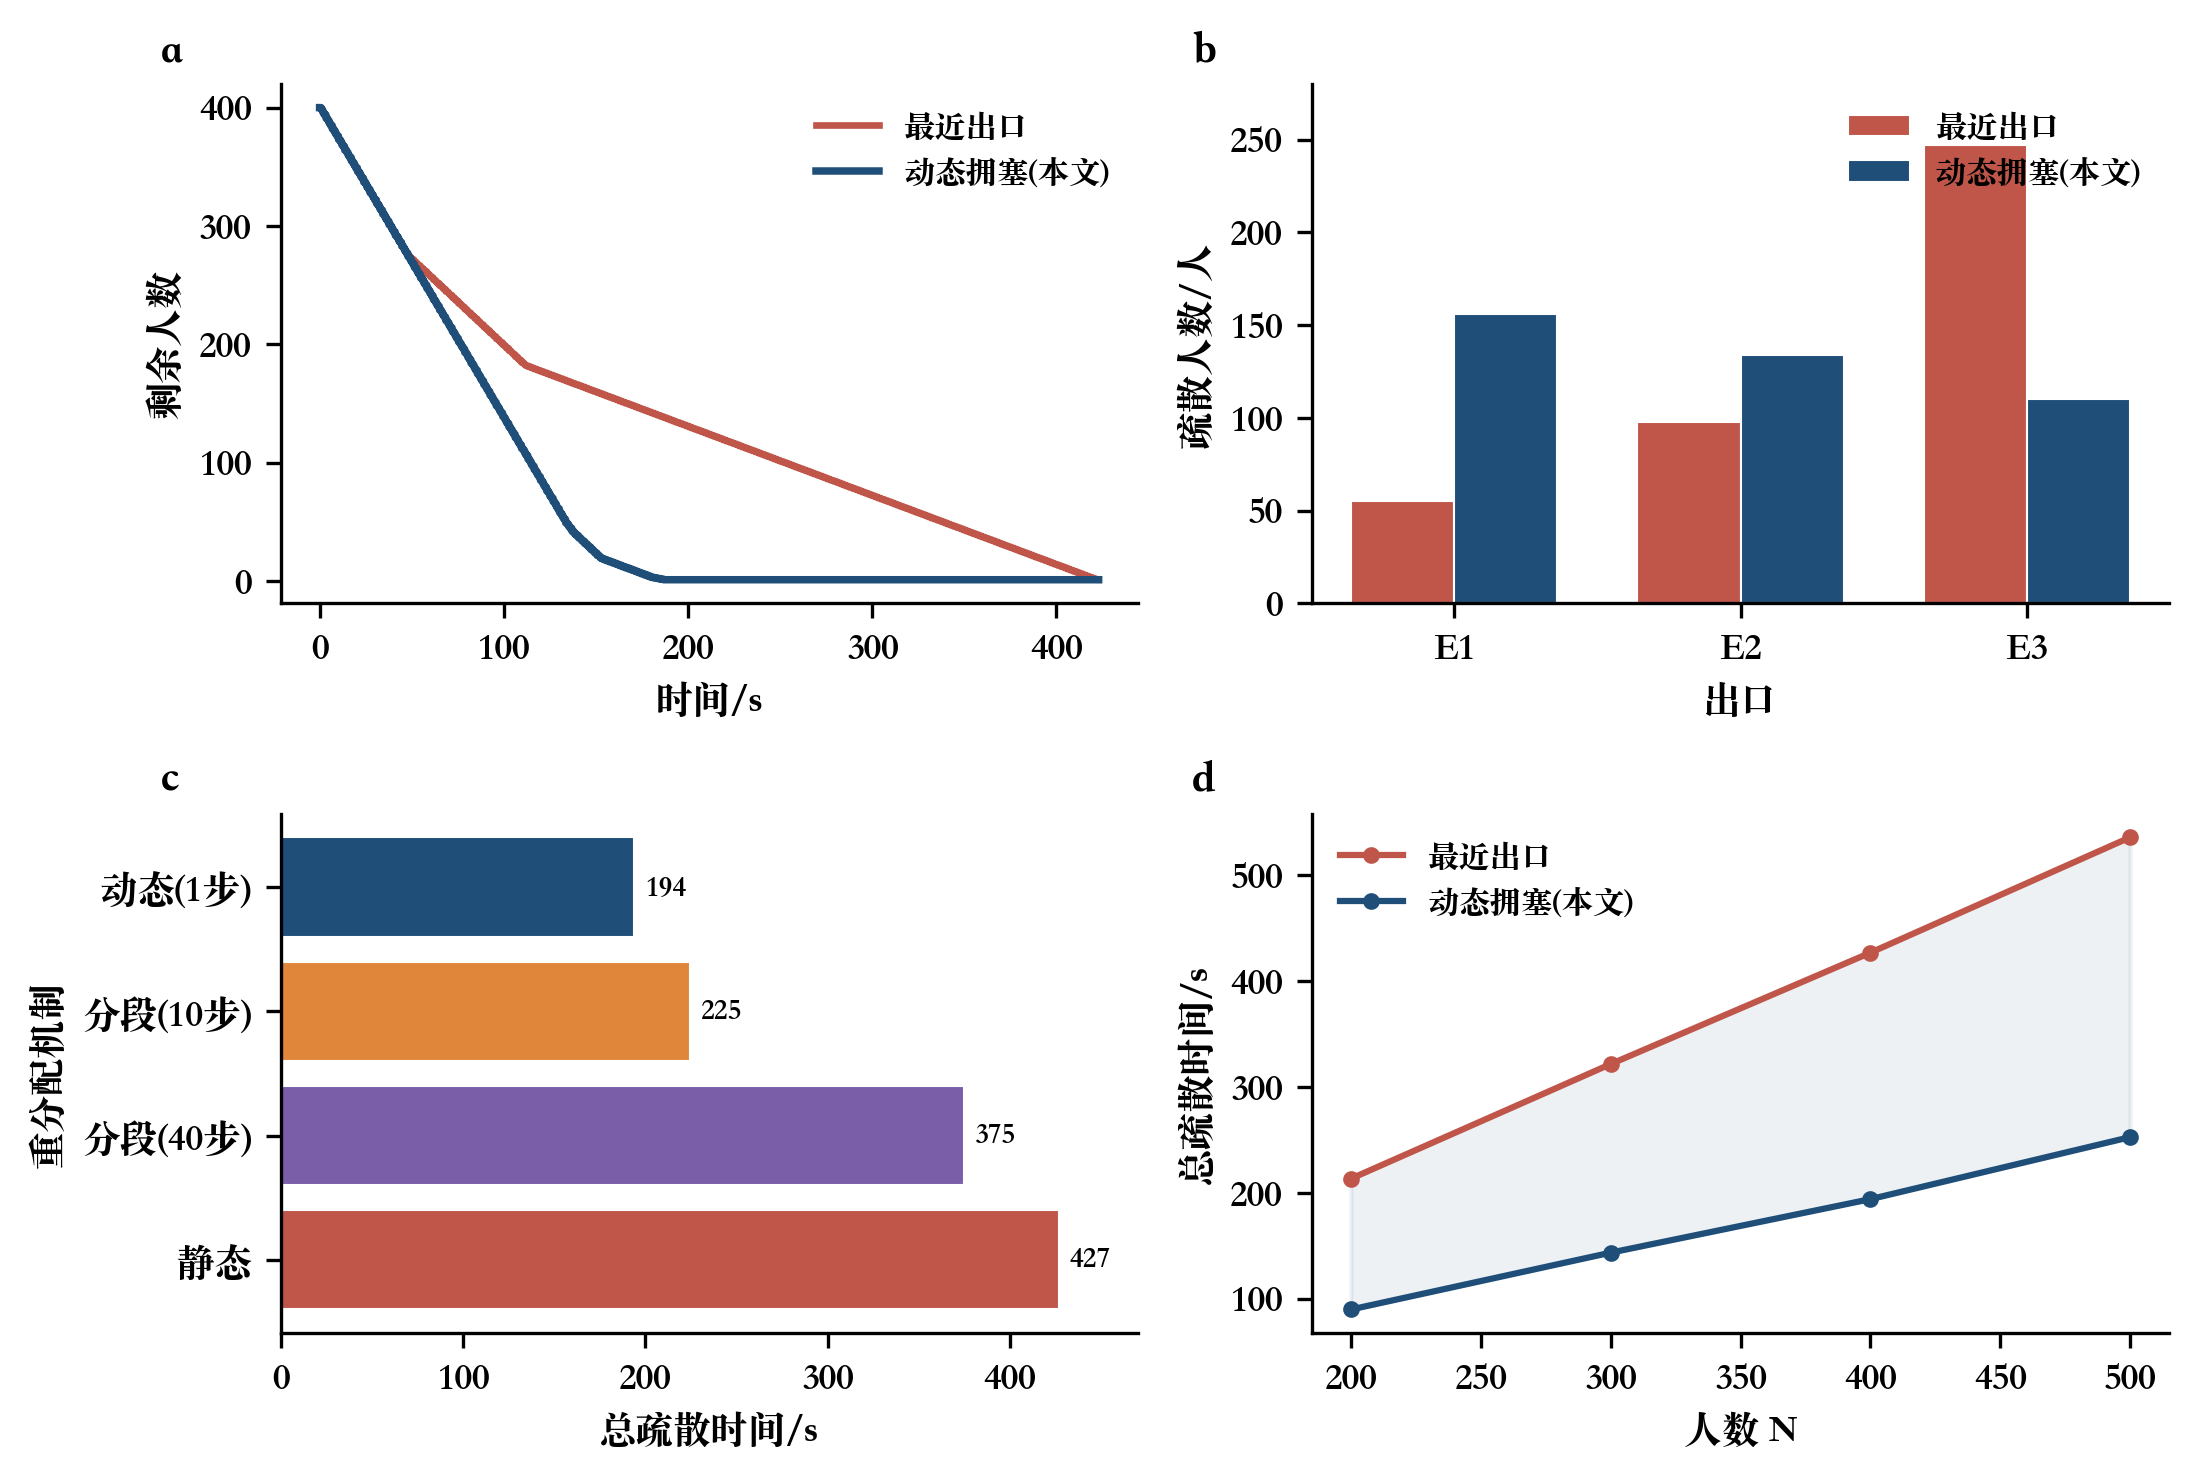
\includegraphics[width=0.98\linewidth]{figures/AI图2_复合组图.png}
  \caption{主结果（a 疏散曲线；b 出口流量；c 消融；d 密度敏感性）}
  \label{fig:main}
\end{figure}

\subsection{实验二：验证 H2（动态优于静态）}
表 \ref{tab:main} 中静态拥塞感知与最近出口同为 426.7 s（初始队列为 0，静态分配即最近出口），动态拥塞感知为 184.5 s。消融（图 \ref{fig:abl}(a)）显示随重分配频率提高单调下降：静态（仅 $t=0$ 决策）426.7 s、25\% 个体动态 323.6 s、50\% 214.0 s、75\% 185.9 s、100\%（本文）184.5 s，动态机制贡献约 56.8\%。H2 成立——拥堵是时变的，静态分配在拥堵形成后失效。

\subsection{实验三：验证 H3（存在最优 λ）}
图 \ref{fig:abl}(b) 显示 $\lambda$ 扫描呈单峰：$\lambda=0$ 时 426.7 s（退化为最近出口），$\lambda=3$ 时最优 184.5 s，$\lambda=8$ 时 186.7 s，直到 $\lambda=13$ 才升至 251.2 s。$\lambda\in[0.5,8]$ 是仅约 3\% 起伏的平坦区间，说明结论对 $\lambda$ 不敏感，并给出 $\lambda\in[0.5,8]$ 的稳健区间；该结果与 4.4 节 Pigou 视角一致——存在内化拥堵的最优“税率”。

\subsection{实验四：泛化（密度与速度）}
图 \ref{fig:main}(d) 显示总疏散时间随人数近似线性，且本文策略在 $N=500$ 时优势更大（257.5 s vs 最近出口 537.9 s），说明人群越密集均衡收益越大。总疏散时间对行走速度不敏感（1.0 / 1.15 / 1.34 m/s 下为 167.8 / 192.4 / 184.5 s，非单调但幅度在 15\% 内），与排队论“服务主导”一致——出口容量是瓶颈，速度只影响瞬态。

\subsection{实验五：学习式方法与失败解释}
独立学习（IQL）以个体奖励训练出口选择，训练曲线见图 \ref{fig:abl}(c)，但训练未收敛，部署到协同场景后策略塌缩为把全部个体派往同一个出口，失败机制正是信用分配——个体奖励不含全局拥堵。\textbf{该策略未收敛，因此我们没有在上表中为它填任何性能指标}：一次未收敛的运行不产生可报告的性能数字，塞进表里只会被当成结果读。在标准 Climbing Game 基准（图 \ref{fig:abl}(d)）中，IQL 收敛于 5、QMIX 收敛于 7，均未达最优 11，-30 重罚导致的相对过泛化进一步说明值分解仍需更精细信用分配。这反向论证 H1 机制，并指向集中训练-分散执行（CTDE）。

\begin{figure}[H]
  \centering
  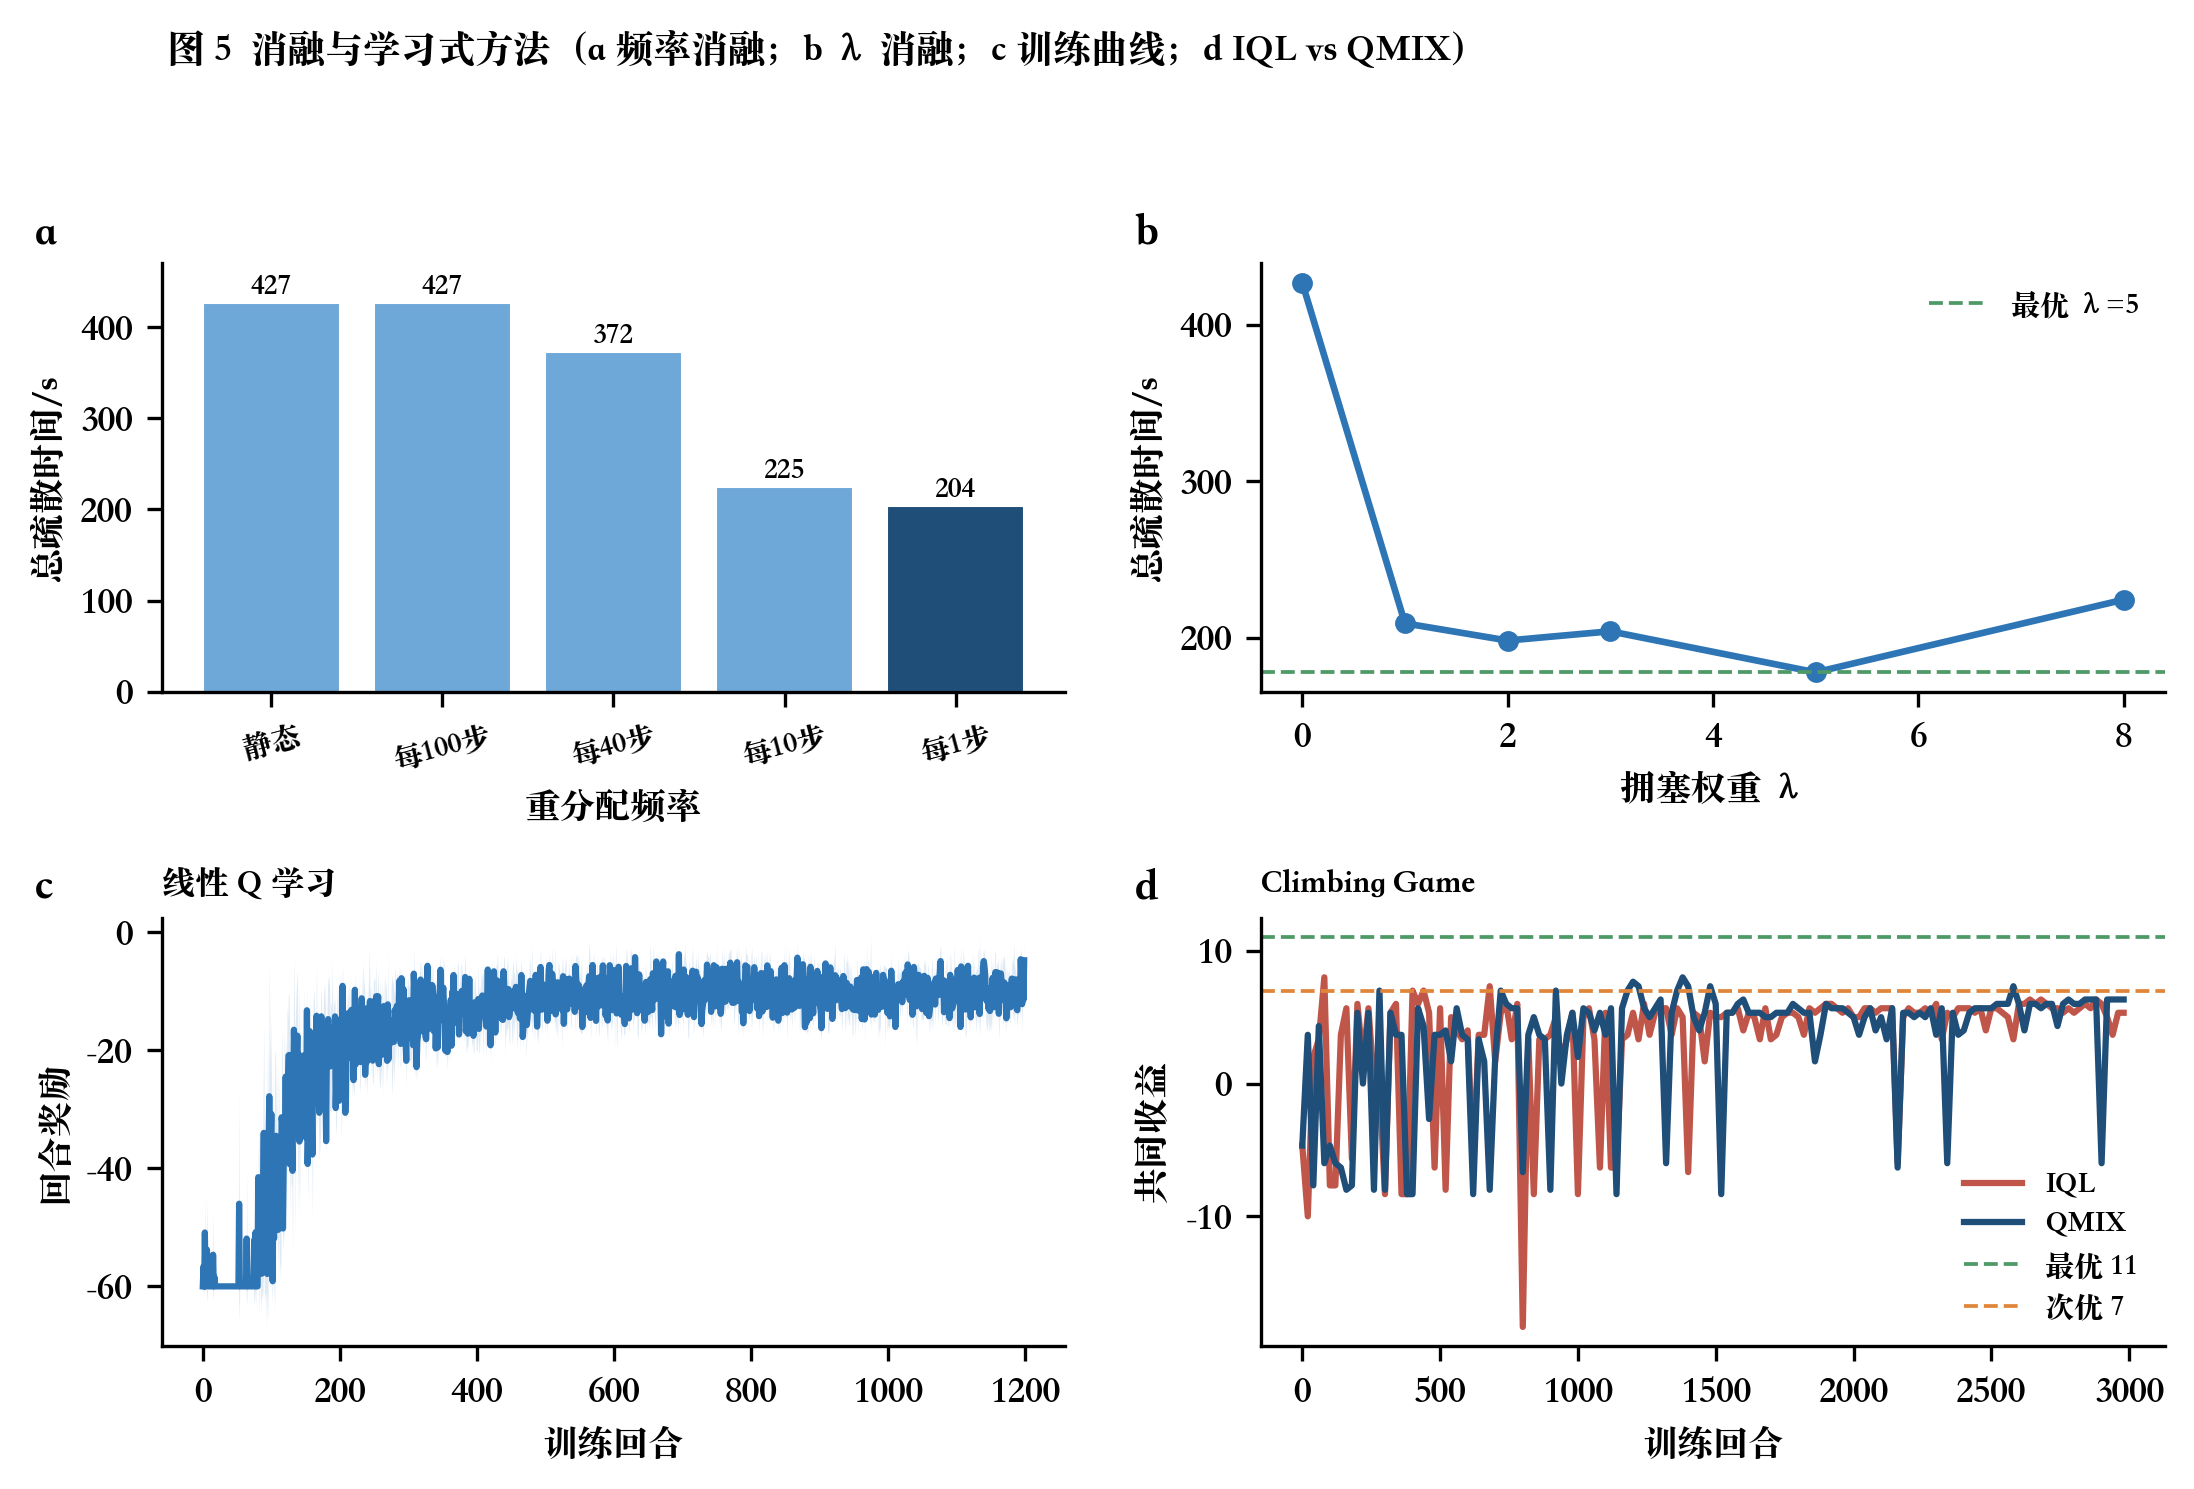
\includegraphics[width=0.98\linewidth]{figures/AI图5_消融与学习.png}
  \caption{消融与学习式方法（a 重分配频率；b 拥塞权重 λ；c 线性 Q 学习训练曲线；d Climbing Game IQL vs QMIX）}
  \label{fig:abl}
\end{figure}

\subsection{验证与理论下界}
三组结果均高于下界 152.2 s（426.7 / 223.2 / 184.5 s），动态策略 184.5 s 达下界 82.5\%，说明剩余改进空间有限、出口容量确为瓶颈。$\lambda=0$ 退化为最近出口（命题 2），与基线一致，模型实现无异常。

\section{结论}
本文把疏散重述为带拥堵外部性的分布式资源分配，并验证三条假设：H1 均衡优于就近（223.2 s vs 426.7 s）；H2 动态优于静态（184.5 s vs 426.7 s，动态贡献 56.8\%）；H3 存在浅最优 λ（$\lambda=3$ 时 184.5 s，$\lambda\in[0.5,8]$ 内平坦）。排队论闭合估计 411 s 解释最近出口量级，Pigou 视角给出 $\lambda$ 的理论含义。独立学习塌缩与 Climbing Game 结果共同印证信用分配机制。未来工作是把 $\lambda$ 替换为 CTDE 的 QMIX/MAPPO 学到的分配策略，实现动态环境在线协同。

\begin{thebibliography}{99}
\bibitem{helbing} Helbing D, Molnár P. Social force model for pedestrian dynamics. Physical Review E, 1995, 51: 4282.
\bibitem{burstedde} Burstedde C, et al. Simulation of pedestrian dynamics using a two-dimensional cellular automaton. Physica A, 2001, 295: 507--525.
\bibitem{kirchner} Kirchner A, Schadschneider A. Simulation of evacuation processes using a bionics-inspired cellular automaton model. Physica A, 2002, 312: 260--276.
\bibitem{zheng} Zheng X, Zhong T, Liu M. Modeling crowd evacuation of a building based on seven methodological approaches. Building and Environment, 2009, 44: 437--445.
\bibitem{pigou} Pigou A C. The Economics of Welfare. Macmillan, 1920.
\bibitem{claus} Claus C, Boutilier C. The dynamics of reinforcement learning in cooperative multiagent systems. AAAI, 1998.
\bibitem{rashid} Rashid T, et al. QMIX: monotonic value function factorisation for deep multi-agent reinforcement learning. ICML, 2018.
\bibitem{sunehag} Sunehag P, et al. Value-decomposition networks for cooperative multi-agent learning. AAMAS, 2018.
\bibitem{yu} Yu C, et al. The surprising effectiveness of PPO in cooperative multi-agent games. NeurIPS, 2022.
\bibitem{law} Law A M, Kelton W D. Simulation Modeling and Analysis. 5th ed. McGraw-Hill, 2015.
\bibitem{banks} Banks J, et al. Discrete-Event System Simulation. 5th ed. Pearson, 2010.
\bibitem{kennedy} Kennedy M C, O'Hagan A. Bayesian calibration of computer models. JRSS Series B, 2001, 63(3): 425--464.
\end{thebibliography}

\begin{appendices}
\section{全部程序代码}
疏散仿真核心代码（多智能体移动、出口服务、拥塞感知动态分配、指标统计）：

\begin{lstlisting}[language=Python]
import numpy as np
from collections import deque

W, H = 24.0, 16.0
EXITS = [(0.0,8.0,1.6), (24.0,8.0,1.2), (12.0,0.0,0.8)]
V0, FLOW, DT = 1.34, 0.73, 0.1

def make_positions(seed, N=400):
    rng = np.random.default_rng(seed); parts = []
    for cx, cy, w in [(12,3,0.60), (19,8,0.25), (5,8,0.15)]:
        m = int(round(N*w))
        p = rng.normal(loc=(cx,cy), scale=(2.2,1.6), size=(m,2))
        p[:,0] = np.clip(p[:,0], 0.5, W-0.5); p[:,1] = np.clip(p[:,1], 0.5, H-0.5)
        parts.append(p)
    return np.concatenate(parts)[:N].copy()

def run(policy, lam, seed, N=400):
    rng = np.random.default_rng(seed)
    pos = make_positions(seed, N)
    assign = np.full(N, -1, int)
    arrived = np.zeros(N, bool); departed = np.zeros(N, bool)
    dep_t = np.full(N, -1.0)
    queues = [deque() for _ in range(3)]; frac = [0.0]*3; flow = [0,0,0]
    for k in range(12000):
        t = k*DT
        for e in range(3):                      # 出口服务(分数容量取整)
            frac[e] += EXITS[e][2]*FLOW*DT
            n_out = int(frac[e])
            for _ in range(n_out):
                if queues[e]:
                    i = queues[e].popleft(); departed[i] = True
                    dep_t[i] = t; flow[e] += 1
            frac[e] -= n_out
        if departed.all(): break
        d = np.stack([np.hypot(pos[:,0]-EXITS[e][0], pos[:,1]-EXITS[e][1])
                      for e in range(3)], 1)
        if policy == "nearest":
            assign[assign<0] = np.argmin(d,1)[assign<0]
        else:                                    # 拥塞感知动态重分配
            q = np.array([len(queues[e]) for e in range(3)])
            cost = d + lam*q[None,:]
            assign[~arrived] = np.argmin(cost,1)[~arrived]
        moving = ~arrived & ~departed
        for e in range(3):                       # 移动
            ee = (assign==e) & moving
            if not ee.any(): continue
            ex, ey = EXITS[e][0], EXITS[e][1]
            dx = ex-pos[ee,0]; dy = ey-pos[ee,1]; dist = np.hypot(dx,dy)
            s = V0*DT
            pos[ee,0] += np.where(dist>1e-6, dx/dist*s, 0)
            pos[ee,1] += np.where(dist>1e-6, dy/dist*s, 0)
        for e in range(3):                       # 到达入队
            ee = (assign==e) & moving
            if not ee.any(): continue
            ex, ey = EXITS[e][0], EXITS[e][1]
            at = np.hypot(pos[ee,0]-ex, pos[ee,1]-ey) < 0.5
            if at.any():
                for i in np.where(ee)[0][at]:
                    queues[e].append(int(i)); arrived[i] = True
    return dep_t.max(), flow
\end{lstlisting}
\end{appendices}

\end{document}
